\documentclass[12pt]{article}

\usepackage{amsfonts,amssymb}
\usepackage[utf8]{inputenc}
\usepackage[russian]{babel}
\usepackage{graphicx}
\usepackage{amsmath}
\usepackage{amsfonts}
\usepackage[ruled, lined]{algorithm2e}
\usepackage{hyperref}

\textheight=220mm
\textwidth=160mm

\newcommand{\sgn}{\operatorname{sgn}}
\newcommand{\argmax}{\operatorname{argmax}}
\newcommand{\NA}{\operatorname{NA}}
\newcommand{\OR}{\operatorname{ or }}
\newcommand{\LCS}{\operatorname{LCS}}
%\DeclareMathOperator{\sgn}{sgn}

\title{\bf Приложение к домашнему заданию № 2 по курсу \\ <<Параллельные
и распределенные вычисления.>>}
\author{А.Е. Оразаев}
\date{}
\begin{document}

\voffset=-20mm
\hoffset=-12mm
\font\Got=eufm10 scaled\magstep2 \font\Got=eufm10

\maketitle

\section{K-means и openmp.}
\paragraph{Ускорение и эффективность}
\begin{center}
    \fbox{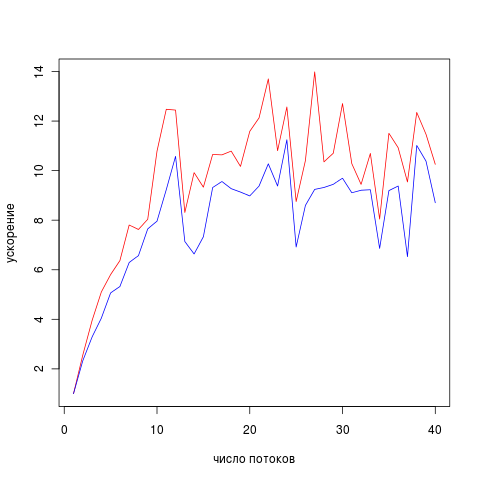
\includegraphics[width=200bp]{hw2.p1/acceleration.png}}
    \fbox{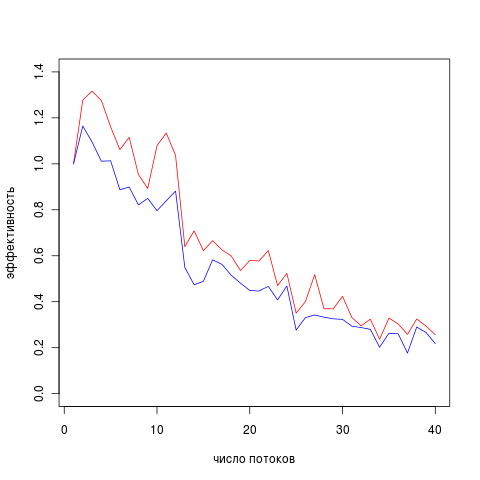
\includegraphics[width=200bp]{hw2.p1/efficiency.png}}
\end{center}
Красной линией отмечены расчеты с минимальными значениями времени, а синей
расчеты со средними значениями.

\section{Игра жизнь.}
\paragraph{Ускорение и эффективность}
\begin{center}
    \fbox{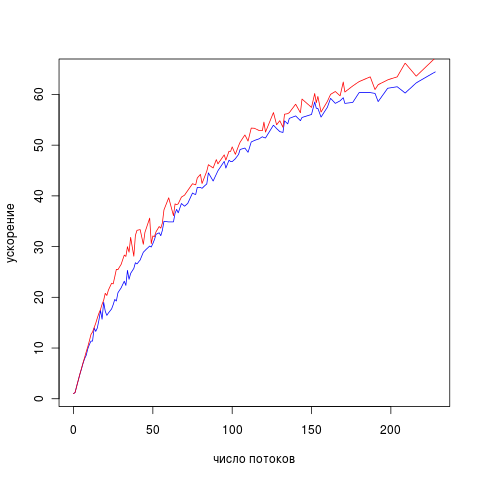
\includegraphics[width=200bp]{hw2.p2/acceleration.png}}
    \fbox{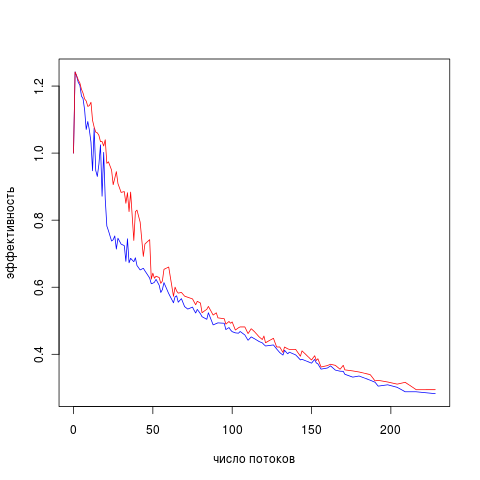
\includegraphics[width=200bp]{hw2.p2/efficiency.png}}
\end{center}
Красной линией отмечены расчеты с минимальными значениями времени, а синей
расчеты со средними значениями.

\end{document}
